\Subhead{1.8.1}{Устойчивость стационарных режимов. Временные методы оценки устойчивости}
\textbf{Определения.} Решение устойчиво по Ляпунову, если достаточно малые начальные отклонения остаются малыми при всех последующих временах. Асимптотическая устойчивость дополнительно требует их стремления к нулю. Для автономного периодического режима сравнивают расстояние до орбиты, разрешая сдвиг фазы. При заданном внешнем периодическом сигнале произвольный сдвиг по фазе уже не является симметрией.


\paragraph{Временная проверка в генераторе.}
Если укороченное уравнение имеет вид $\dot A=f(A)$, то около $A_*$: $\delta\dot A=f'(A_*)\delta A$. Возврат требует $f'(A_*)<0$. Равносильно, за период малое отклонение умножается на $\rho=\exp[f'(A_*)T]$, $|\rho|<1$. На графике отображения $A_{n+1}=P(A_n)$ это пересечение с диагональю с наклоном $|P'|<1$. Так один режим можно оценить по времени восстановления, по показателю или по мультипликатору.
\paragraph{Равновесие и показатели роста.}
В окрестности стационарного состояния $\dot{\bm\xi}=J\bm\xi$, $\bm\xi(t)=\e^{Jt}\bm\xi(0)$. Если все $\operatorname{Re}\lambda_j(J)<0$, равновесие гладкой нелинейной системы локально асимптотически устойчиво; если хотя бы одна действительная часть положительна, неустойчиво. При нулевых действительных частях линейный тест не решает задачу. Даже отрицательные показатели могут сопровождаться временным усилением нормы в ненормальной матрице; это не экспоненциальная неустойчивость, но может выводить за пределы локальной области.

У двумерной системы критерий $\operatorname{tr}J<0$, $\det J>0$ эквивалентен отрицательным действительным частям обоих корней. Для вещественного кубического характеристического полинома $s^3+a_1s^2+a_2s+a_3$ критерий Рауса--Гурвица:
\begin{equation}
 a_1>0,\quad a_2>0,\quad a_3>0,\quad a_1a_2>a_3.
\end{equation}
Это удобно, когда выписывание самих корней ничего не проясняет. Критерий относится к непрерывному времени и полиному с положительным старшим коэффициентом.

\paragraph{Энергетический метод.}
Функция Ляпунова $V(\bm\xi)>0$, $V(0)=0$, $\dot V\leq0$ позволяет доказать устойчивость без интегрирования. Для пассивного осциллятора $V=E$, $\dot E=-2m\gamma v^2$. Хотя производная не строго отрицательна на линии $v=0$, при $\gamma,k>0$ единственное движение, целиком остающееся на ней, --- равновесие; отсюда следует притяжение. Для активной системы энергия не обязана монотонно убывать, и её саму нельзя автоматически использовать как такую функцию.
\begin{center}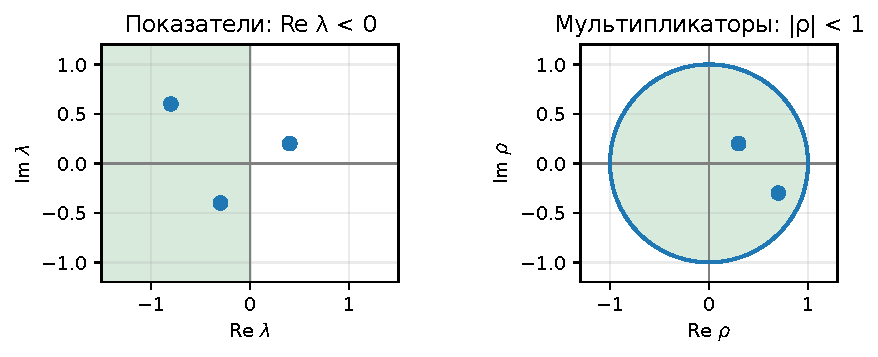
\includegraphics[width=0.72\linewidth]{figures/stability.pdf}\end{center}
